\documentclass[11pt,openright,a4paper]{article}
\usepackage{fancyhdr}
\usepackage{datetime}
\usepackage[left=25mm,right=25mm,top=35mm,bottom=35mm,footskip=0.5in]{geometry}
% %%
%% Package includes to provide the basic style
%%
\usepackage{harvard}    % Uses harvard style referencing
\usepackage{graphicx}   % Permits import of various graphics formats
\usepackage{hyperref}   % Provides hyperlinks to sections automatically
\usepackage{pdflscape}  % Provides landscape mode for end code listings
\usepackage{multicol}   % Provides ability to split output into columns
\usepackage{listings}   % Provides styled code listings
\usepackage{titlesec}
\usepackage[margin=35mm,footskip=0.5in]{geometry}
\usepackage{tabularx}
\usepackage{tabulary}
\usepackage{multirow}
\usepackage{color}
\usepackage[table]{xcolor}
\usepackage{caption, subcaption}
\usepackage{amssymb, amsmath, empheq}
\lstset{language=Python}
\usepackage{array}
\usepackage{longtable}
\usepackage{subfiles}
\usepackage{float}
\usepackage{longtable}

\graphicspath{ {images/} {lit_review/images/} {images/tech/} {images/methodology/} {images/results/} }
% \numberwithin{equation}{chapter}

\let\subsectionautorefname\sectionautorefname
\let\subsubsectionautorefname\sectionautorefname

% % set margin
% \geometry{
%   a4paper,
%   top=25mm,
%   bottom=35mm
% }

%%
%% Set some page size changes from the standard article class
%%
\usepackage{calc}
\setlength{\parskip}{6pt}
\setlength{\parindent}{0pt}
\addtolength{\hoffset}{0.5cm}
\addtolength{\textwidth}{0.5cm}

% set section depth
\setcounter{tocdepth}{4}
\setcounter{secnumdepth}{5}

% set chapter format
%\titleformat{\chapter}[hang]{\LARGE\bfseries}{\thechapter\hspace{20pt}}{0pt}{\LARGE\bfseries}
%\titlespacing{\chapter}{0pt}{0pt}{5pt}

%%
%% Format definitions for the style
%%
\bibliographystyle{agsm}  %{alpha}
\citationstyle{dcu}
\pagestyle{headings}
\fussy


%%
%% Definitions to provide layout in the dissertation title pages
%%
\newenvironment{spaced}[1]
  {\begin{minipage}[c]{\textwidth}\vspace{#1}}
  {\end{minipage}}


\newenvironment{centrespaced}[2]
  {\begin{center}\begin{minipage}[c]{#1}\vspace{#2}}
  {\end{minipage}\end{center}}


%%
%% New column header command
%% 
\newcolumntype{Z}{ >{\centering\arraybackslash}X }
\newcolumntype{M}[1]{ >{\centering\arraybackslash}m{#1}}


% declaration
\newcommand{\declaration}[2]{
  \thispagestyle{empty}
  \begin{spaced}{4em}
    \begin{center}
      \LARGE\textbf{#1}
    \end{center}
  \end{spaced}
  \begin{spaced}{3em}
    \begin{center}
      Submitted by: #2
    \end{center}
  \end{spaced}
  \begin{spaced}{5em}
    \section*{COPYRIGHT}

    Attention is drawn to the fact that copyright of this dissertation rests
    with its author. The Intellectual Property Rights of the products
    produced as part of the project belong to the author unless otherwise specified
    below, in accordance with the University of Bath's policy on intellectual property 
   (see http://www.bath.ac.uk/ordinances/22.pdf).

    This copy of the dissertation has been supplied on condition that anyone
    who consults it is understood to recognise that its copyright rests with its
    author and that no quotation from the dissertation and no information
    derived from it may be published without the prior written consent of
    the author. \\ \\

    \section*{DECLARATION}
    This dissertation is submitted to the University of Bath in accordance
    with the requirements of the degree of Bachelor of Science in the
    Department of Computer Science. No portion of the work in this dissertation
    has been submitted in support of an application for any other degree
    or qualification of this or any other university or institution of learning.
    Except where specifically acknowledged, it is the work of the author.
  \end{spaced}

  \begin{spaced}{5em}
    Signed:
  \end{spaced}
  }


% consultation
\newcommand{\consultation}[1]{%
\thispagestyle{empty}
\begin{centrespaced}{0.8\textwidth}{0.4\textheight}
\ifnum #1 = 0
This dissertation may be made available for consultation within the
University Library and may be photocopied or lent to other libraries
for the purposes of consultation.
\else
This dissertation may not be consulted, photocopied or lent to other
libraries without the permission of the author for #1 
\ifnum #1 = 1
year
\else
years
\fi
from the date of submission of the dissertation.
\fi
\vspace{4em}

Signed:
\end{centrespaced}
}

%%
%% END OF DEFINITIONS
%%


\usepackage{amsmath}
\usepackage{hyperref}
\usepackage{amsbsy}
\usepackage{graphicx}
\usepackage{float}

\usepackage[english]{babel}
\usepackage[backend=bibtex,sorting=none,style=ieee]{biblatex}
\bibliography{task1bib}

\graphicspath{ {images/} }
\usepackage{graphicx}

% header
\pagestyle{fancy}
\fancyhf{}
\lhead{CM50426 Machine Learning \& AI \\ Alan Lau}
\rhead{Task 1 \\ Semester 1, 2016-17}
\cfoot{\thepage}

\setlength{\parindent}{0em}
\setlength{\parskip}{1em}
\numberwithin{equation}{section}

\abovedisplayskip=12pt plus 3pt minus 9pt
\abovedisplayshortskip=0pt plus 3pt
\belowdisplayskip=12pt plus 3pt minus 9pt
\belowdisplayshortskip=7pt plus 3pt minus 4pt

\usepackage[font=small,labelfont=bf]{caption}

\begin{document}

%%%%%%%%%%%%%
\section{Introduction} \label{sec:intro}
%%%%%%%%%%%%%
Unsupervised learning algorithms attempt to learn the hidden structure of a given dataset without any labels or knowledge of the distributions of the data. A prominent usage of such algorithms is for clustering. A given set of datapoints is split into groups based on their underlying patterns. By learning the required parameters, points can be assigned to clusters and distributions can be observed.

Broadly speaking, there are three types of clustering algorithms, namely, centroid-based, distribution-based and density-based. A centroid-based algorithm, such as \textit{K}-means, uses a single mean vector to represent each cluster, and assign points to clusters in a binary fashion. On the other hand, Gaussian Mixture Model (GMM) is a prime example of a distribution-based clustering algorithm. It mixes together multivariate Gaussian distributions and uses probability theories to derive soft assignments to the corresponding distributions. 

We shall further discuss \textit{K}-Means and GMM, and a generic method called Expectation-Maximisation that facilitates these two algorithms.


%%%%%%%%%%%%
\section{Expectation-Maximisation (EM)} \label{sec:em}
%%%%%%%%%%%%

\begin{equation} \label{eq:em-prob}
    Pr\left( \boldsymbol{x} | \boldsymbol{\theta} \right) = 
    \int Pr\left( \boldsymbol{x},\boldsymbol{h} | \boldsymbol{\theta} \right) \; d\boldsymbol{h}
\end{equation}

\begin{equation} \label{eq:em-max}
    \hat{\boldsymbol{\theta}} = 
        \underset{\boldsymbol{\theta}}{\mathrm{argmax}}
        \left[ \sum_{i=1}^{I} \log \left[ 
            \int Pr\left( \boldsymbol{x}_{i},\boldsymbol{h}_{i} | \boldsymbol{\theta} \right) \; d\boldsymbol{h}_{i} 
            \right] 
        \right]
\end{equation}

EM is a generic algorithm that is used to fit parameters, $\boldsymbol{\theta}$, of models in the form of \autoref{eq:em-prob}. The algorithm aims to find the arguments that maximises the marginalised joint probability facilitated by the hidden variable, $\boldsymbol{h}$, as shown in \autoref{eq:em-max}. One could directly apply maximum likelihood (ML) and find $\boldsymbol{\theta}$ by maximising the log likelihood of $Pr\left( \boldsymbol{x}| \boldsymbol{\theta} \right)$. This eliminates the need of $\boldsymbol{h}$ which makes the calculation more straight-forward, but no closed form solution will be found for the models we are concerned of.

It is a two-step process - \textit{E-step} and \textit{M-step}:
\begin{itemize}
    \item \textit{E-step} (expectation step) updates the probabiliy distributions, $q_{i}\left(\boldsymbol{h}_{i} \right)$, while fixing $\boldsymbol{\theta}$ to maximise the lower bound; and,
    \item \textit{M-step} (maximisation step) updates the parameters, $\boldsymbol{\theta}$, while fixing $q_{i}\left(\boldsymbol{h}_{i} \right)$ to maximise the lower bound. 
\end{itemize}

The E-step and M-step runs in this order for once each in every iteration. The algorithm will iterate until it converges , which is guaranteed by the bounds of the algorithm. In other words, the algorithm will iterate until a local maximum in the likelihood function is reached. The goal for both steps is to increase the lower bound $\mathcal{B}\left[q_{i}\left(\boldsymbol{h}_i\right),\boldsymbol{\theta} \right]$ while not exceeding the upper bound, which is the sum of the log joint likelihoods of a point and its corresponding $\boldsymbol{h}$ value. 


\begin{figure}[H]
  \centering
  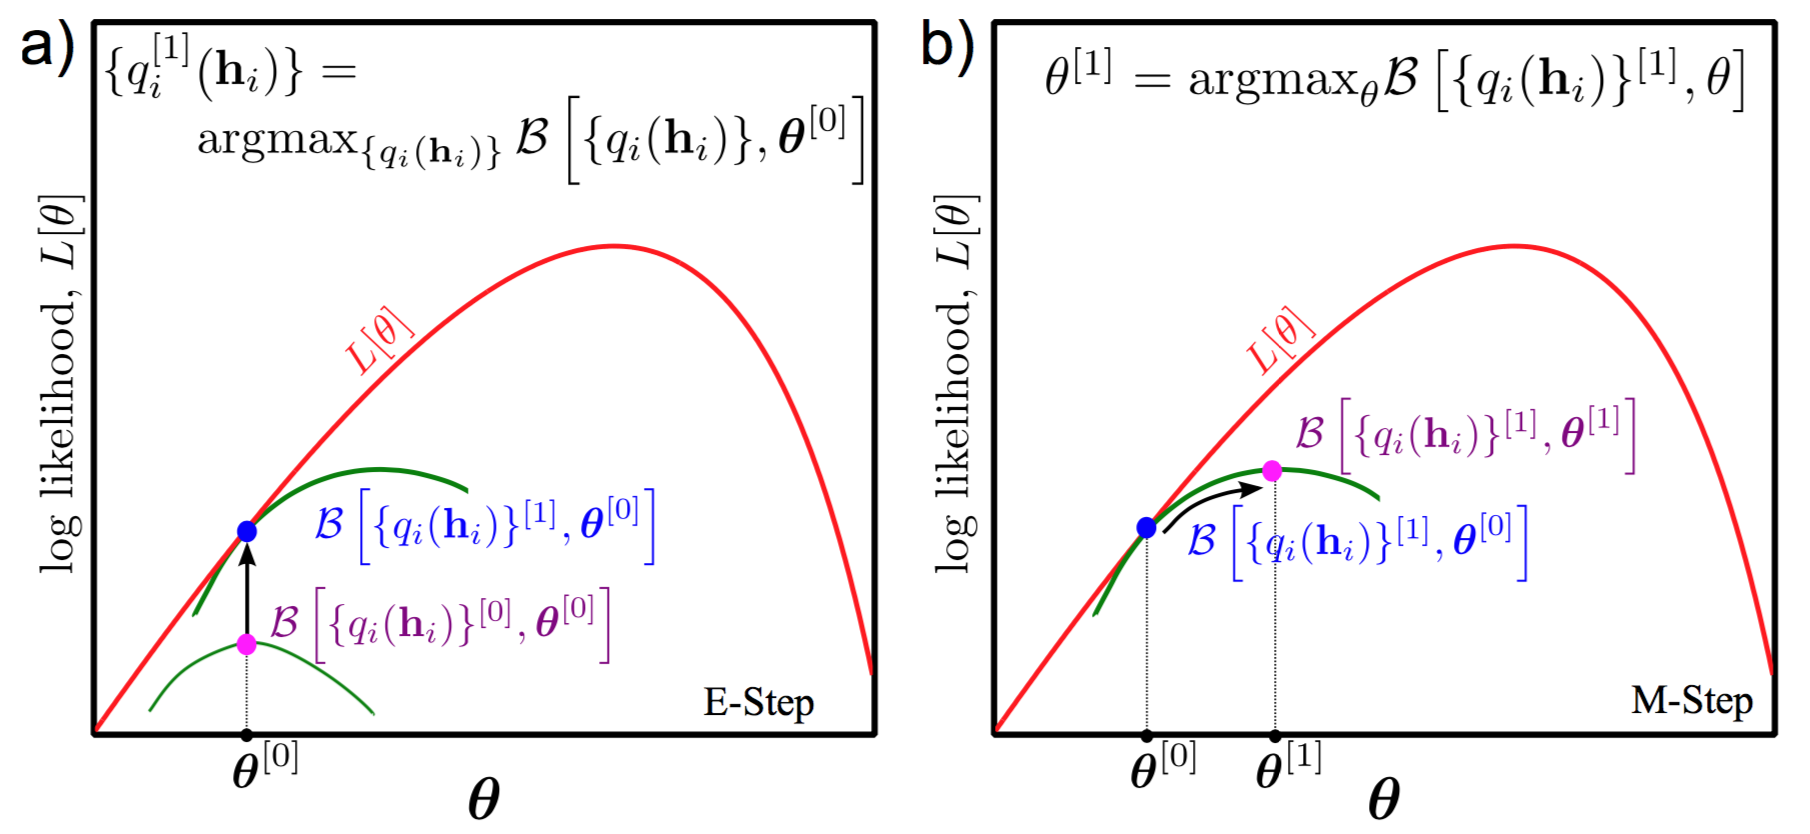
\includegraphics[width=0.7\textwidth]{em-overview}
    \caption{(left) The graph shows an E-step, where manipulating the probability distributions changes all values of the lower bound for every $\boldsymbol{\theta}$, hence the whole curve moves towards the red curve, which is the actual log likelihood curve. (right) The graph shows an M-step, where the $\boldsymbol{\theta}$ is changed while fixing $q_{i}(\boldsymbol{h}_{i}$ to improve the estimate from the blue dot to the purple dot. (Figure taken from \cite{prince}.)}
  \label{fig:em-overview}
\end{figure} 


%%%%%%%%%%%%
\section{\textit{K}-means} \label{sec:km}
%%%%%%%%%%%%
The goal of \textit{K}-means is that given $K$ number of clusters, assign each point to a cluster centre at this iteration (known as a prototype) , $\boldsymbol{\mu}_k$, where the distance between the point and the this centre is the smallest compared to the others. The means of the points assigned to each cluster form the new prototypes, and the process continues until it converges. This resembles the EM structure where we first fix the prototypes to update responsibilities, then the other way round.

\begin{equation} \label{eq:km-obj-func}
    J = \sum_{i=1}^{I} \sum_{k=1}^{K} r_{ik} \left|\left| \boldsymbol{x}_{i} - \boldsymbol{\mu}_{k} \right|\right|^2
\end{equation}

More formally, we define the objective function of the model as \autoref{eq:km-obj-func}, with $r_{ik}$ being the responsibility and the latter part the Euclidean distance between the datapoint and prototype concerned. We aim to minimise this function through the EM procedures.

\begin{equation} \label{eq:km-e-step}
    r_{ik} = 
    \begin{cases}
        1 \quad \mathrm{if} \, k = \mathrm{argmin}_j
                            \left|\left|\boldsymbol{x}_{i} - \boldsymbol{\mu}_{k} \right|\right| \\
        0 \quad \mathrm{otherwise}
    \end{cases}
\end{equation}

In the E-step, we update the responsibilities while fixing the prototypes. Here, the responsibilities act as `weights', telling how likely a datapoint belongs to each of the clusters. The sum of all responsibilities for each datapoint across all clusters should always equal to 1. In fact, for \textit{K}-means, this is simply a binary assignment, as datapoints are hard-assigned to one cluster only, as illustrated in \autoref{eq:km-e-step}.

\begin{equation} \label{eq:km-m-step}
    \boldsymbol\mu_{k} = \frac{\sum_i r_{ik}\boldsymbol{x}_i}{\sum_i r_{ik}}
\end{equation}

In the M-step, using the new responsibility assignments from the E-step, we calculate the prototypes, as shown in \autoref{eq:km-m-step}. Essentially, it is simply the mean of all the datapoints of a cluster.

The EM steps are repeated until the prototypes remains unchanged. Then, the final centroids are found. The dataset is grouped together by them, for which they act as the means of the $K$ different clusters.

%TODO: How to initialise 


%%%%%%%%%%%%
\section{Guassion Mixture Model (GMM)} \label{sec:gmm}
%%%%%%%%%%%%

% TODO
% responsibilities
% How K-means is a specific case of GMM
% why EM but not direct ML
% what is it good for 

\begin{equation}
    \label{eq:norm-dist}
    \mathrm{Norm}_{x}\left[\boldsymbol{\mu},\boldsymbol{\Sigma}\right] = 
        \frac{1}{\left( 2 \pi \right)^\frac{d}{2}}
        |\boldsymbol\Sigma|^{-\frac{1}{2}} 
        \,\mathrm{exp}\, 
        \left\{-
            \frac{1}{2}
            \left(\boldsymbol{x}-\boldsymbol{\mu}\right)^\mathrm{T} 
            \boldsymbol{\Sigma}^{-1}
            \left(\boldsymbol{x}-\boldsymbol{\mu}\right)
        \right\}
\end{equation}

\begin{equation} \label{eq:gmm}
    Pr\left(\boldsymbol{x} | \boldsymbol{\theta}\right) =
    \sum_{k=1}^K \lambda_k \mathrm{Norm}_{x}\left[\boldsymbol{\mu}_k, \boldsymbol{\Sigma}_k\right]
\end{equation}

We define the multivariate normal distribution in \autoref{eq:norm-dist}, with means, $\boldsymbol\mu$, and covariance matrices, $\boldsymbol\Sigma$, as parameters. A mixture of Gaussian is the weighted sum of all $K$ normal distributions, also known as linear super-position of Gaussians, as illustrated by \autoref{eq:gmm}. Here, $K$ represents the number of components given to fit the the model to the data. The weights, $\lambda$, can also be viewed as the priors to the probability.

% TODO: add Cat[lambda] stuff

A mixture of Gaussian poses some constraints. Like $K$-means, the weights, $\lambda$, for each datapoint across all components should sum to 1, which $Pr\left(\boldsymbol{x}\right)$. Also, $\boldsymbol{\Sigma}$ needs to be positive definite matrices for $\mathrm{Norm}_x$ to work.

As mentioned in \autoref{sec:em}, it is not possible to obtain a closed form solution when differentiate with respect to $\boldsymbol{\theta}$ and equating that to zero by directly applying maximum likelihood. A non-linear optimisation approach could be attempted, but it would be rather difficult to maintain the aforementioned parametric contraints. The EM approach provides a simple yet powerful method to fit against a multi-dimensional dataset. 

\begin{equation} \label{eq:gmm-back}
    \begin{aligned}
        Pr\left(\boldsymbol{x}|\boldsymbol{h},\boldsymbol{\theta}\right) 
            &= \mathrm{Norm}_x\left[\boldsymbol{\mu}_h,\boldsymbol{\Sigma}_h\right] \\ 
        Pr(\boldsymbol{h}|\boldsymbol{\theta}) &= \mathrm{Cat}_h\left[ \boldsymbol{\lambda}\right]
    \end{aligned}
\end{equation}

Going back to \autoref{eq:gmm} - the probability distribution is derived by considering the hidden variable, $\boldsymbol{h}$. By defining \autoref{eq:gmm-back}, we can define $Pr(\boldsymbol{x} | \boldsymbol{\theta})$ as the marginalisation between $\boldsymbol{x}$ and $\boldsymbol{\lambda}$.

In this way, we can draw samples using $Pr(\boldsymbol{x},h)$. Discarding $h$ leaves the samples. We also observe that the hidden variable here is the weights for the model, which describes the responsibilities to each normal distribution for each datapoint. 

\subsection{Applying EM to GMM} \label{ssec:gmm-em}

\begin{figure}[H]
  \centering
  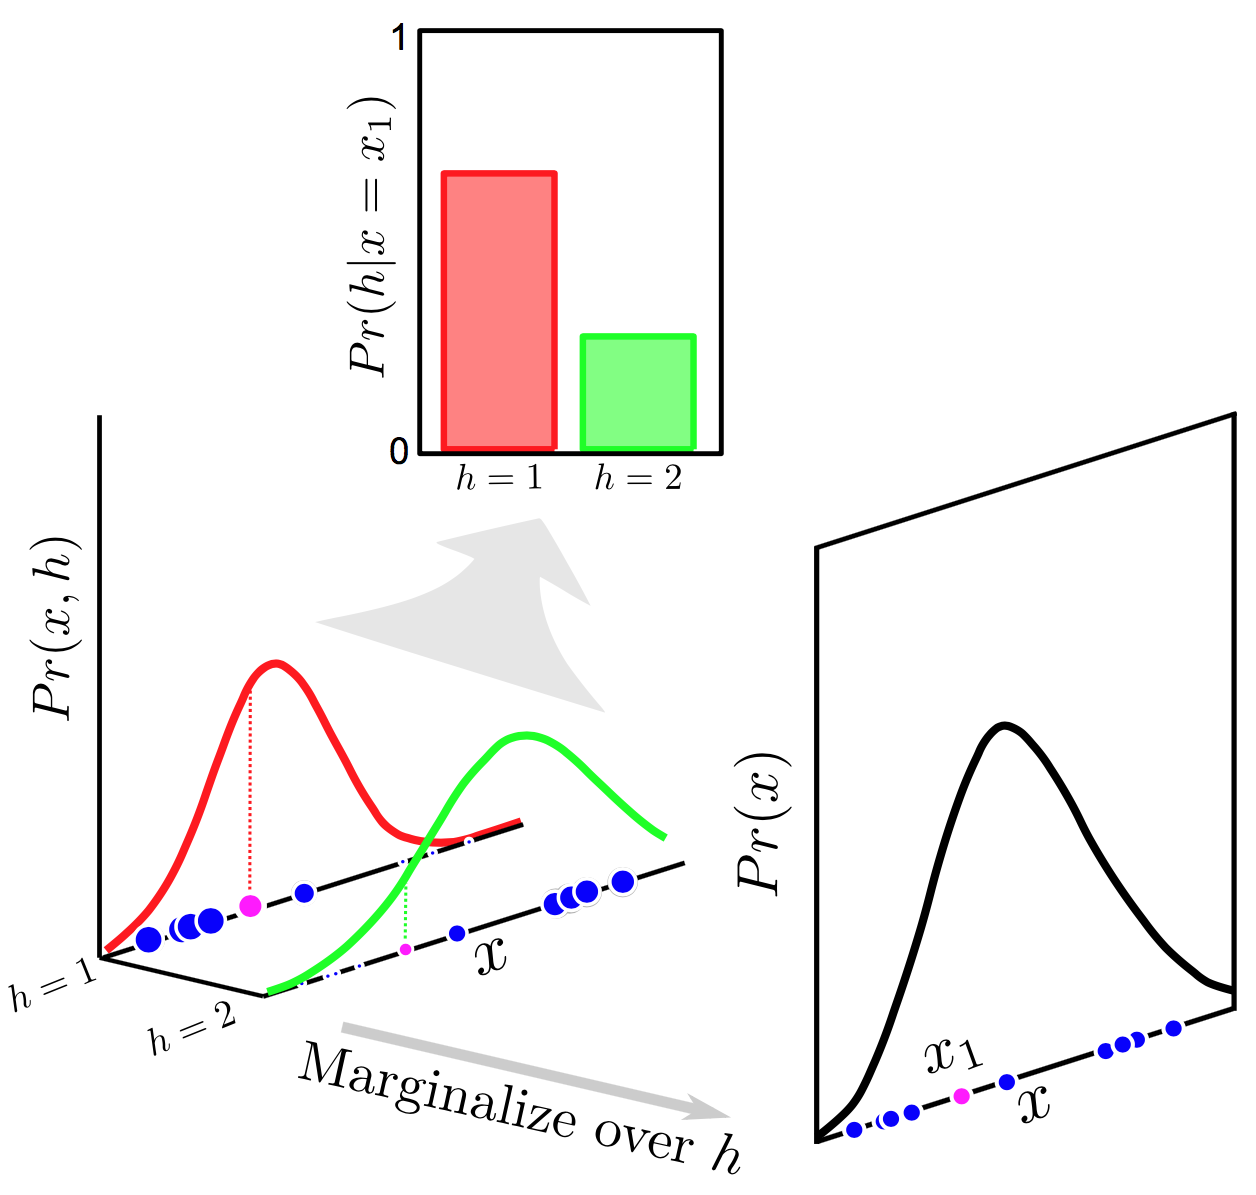
\includegraphics[width=0.5\textwidth]{gmm-e-step}
    \caption{By calculating the posterior distribution, $Pr(h_i|\boldsymbol{x}_i$, we obtain a set of responsibilities. In this example, we can see that component 1 has a much higher responsibility for the datapoint $\boldsymbol{x}_i$ than component 2. (Taken from \cite{prince})}
  \label{fig:gmm-e-step}
\end{figure} 


\begin{equation}
    \label{eq:gmm-e-step}
    q_i\left(h_i\right) = Pr\left(h_i=k|\boldsymbol{x}_i, \boldsymbol{\theta}^{\left[t\right]}\right) = 
    r_{ik} = 
    \frac{\lambda_{k}\,\mathrm{Norm}_{x_i}\left[\boldsymbol{\mu_k},\boldsymbol{\Sigma_k} \right]}
        {\sum_{k'} \lambda_{k'}\,\mathrm{Norm}_{x_i}\left[\boldsymbol{\mu_{k'}},\boldsymbol{\Sigma_{k'}} \right]}
\end{equation}

There is now sufficient information for us to consider the EM approach to learn these parameters, namely, responsibilities, means and covariance matrices under the GMM. In the E-step, we are to calculate the responsibilities. Recall that in this step, we are to evalutate the probability distributions while fixing the other parameters and the datapoint $\boldsymbol{x}_i$. 

As shown in \autoref{eq:gmm-e-step}, it is in fact the posterior probability distribution $Pr(h_i|\boldsymbol{x}_i)$ that is being calculated. Unlike $K$-Means, these are not binary (i.e. not hard) assignments. The points are softly assigned to coponents, in that the responsibility from each component is taken into account. These probabilities will help decide which component $k$ is most likely to be responsible for the datapoint $\boldsymbol{x}_i$.


\begin{figure}[H]
  \centering
  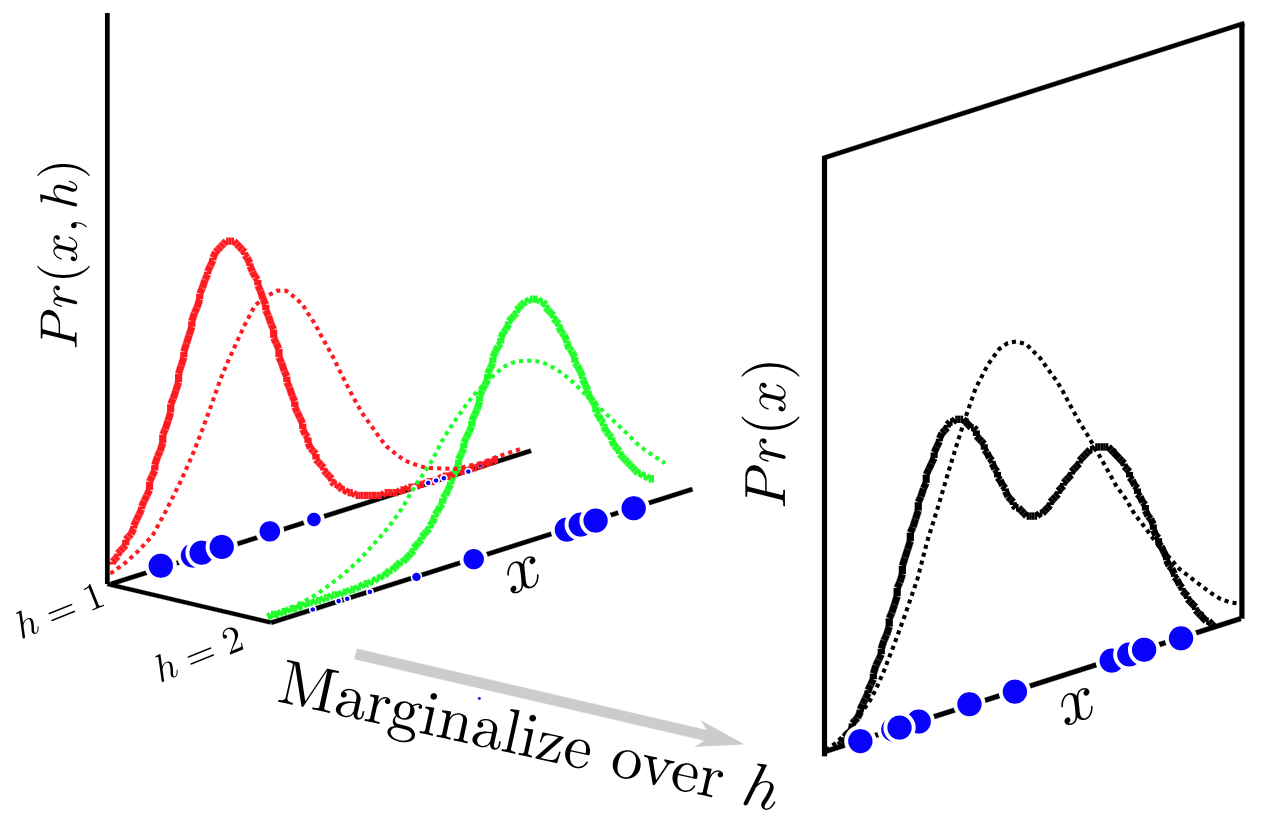
\includegraphics[width=0.5\textwidth]{gmm-m-step}
    \caption{Observe that as the parameters are updated in the M-step, the shape distributions changes, and changing the final mixture model. (Taken from \cite{prince})}
  \label{fig:gmm-m-step}
\end{figure} 

\begin{equation}
    \label{eq:gmm-m-step}
    \begin{aligned}
        m_{k} &= \sum_{i=1}^{I} r_{ik} \\ 
        \lambda_{k}^{\left[t+1\right]} &= \frac{m_{k}}{\sum_{j=1}^{K} m_{j}} \\
        \boldsymbol\mu_{k}^{\left[t+1\right]} &= \frac{\sum_{i=1}^{I} r_{ik} \boldsymbol{x}_{i}}{m_{k}} \\
        \boldsymbol\Sigma_{k}^{\left[t+1\right]} &= 
            \frac{\sum_{i=1}^{I} r_{ik} 
                    \left(\boldsymbol{x}_{i} - \boldsymbol{\mu}_{k}^{\left[t+1\right]}\right)
                    \left(\boldsymbol{x}_{i} - \boldsymbol{\mu}_{k}^{\left[t+1\right] }\right)^\mathrm{T}}
                {m_{k}}
    \end{aligned}
\end{equation}

In the M-step, we are to update all the parameters based on the newly calculated responsibilies in the E-step, as illustrated in \autoref{eq:gmm-m-step}, which can be interpreted easily. By tweaking the parameters, shown in \autoref{fig:gmm-m-step}, the shape of the individual normal distributions change, which in turns changes the overall mixture. 

The responsibilies is crucial in updating the parameters. The influence of a datapoint on each component depends on them. For instance, the cluster means, $\boldsymbol\mu_{1...k}$, the weighted mean over the datapoints are computed, where these weights are the corresponding component responsibilities. Similarly, this is true for the covariance matrices.

The closed form solutions, the guarantee observations of the constraints on parameters and the ability to workaround missing data makes EM a great method to be used by GMM. As mentioned before, simply by applying maximum likelihood would not create closed form solutions, which makes it very difficult to observe the contraints while trying to achieve the maximum likelihood.

\newpage
%%%%%%%%%%%%%
\section{Discussions} \label{sec:dis}
%%%%%%%%%%%%%
\subsection{Linking $K$-means and GMM} \label{ssec:dis-link}
The EM framework works very well under $K$-means and GMM. It provides closed form solutions and guarantees convergence for both algorithms. EM aside, one can see that there are striking similarities between the two. The goal for both is to create clusters based on the datapoints, using a very similar set of parameters.

However, there are are a few minor but noticable differences between the algorithms. For instance, $K$-means of hard and soft assignments to clusters in $K$-means and GMM respectively. This means that $K$-means 

Based on these similarities and differences, one could suggest that $K$-means is a specific case of GMM, in that the hard assignment and the lack of considerations of covariance makes it bias towards far apart, spherical-based datasets. On the other hand, GMM provides a more flexible solution. The addition of covariance matrices in GMM enables a tilted, eclipse shape.

\subsection{Initialisation} \label{ssec:dis-init}
One important problem to consider is when to is how to initialise either of the methods

\subsection{}



%%%%%%%%%%%%%
\section{Results}
%%%%%%%%%%%%%
% TODO
% dimensionality
% scalability
% gmm - init random VS init with K-means

\section{Future Work}

\section{Python Scripts Documentation}

\printbibliography

\end{document}
